%Korrekturgelesen: Ann-Sophie Dietrich
\chapter{Ausblick}
\label{ausblick}
In der nächsten Ausbaustufe soll ein Rasberry Pi zwischen den Mikrocontroller
und die Webseite geschalten werden. Dieses System eröffnet eine Vielzahl
neuer Möglichkeiten, so können von einer Webseite aus mehrere Pollin Net-IO
Boards verwaltet werden und die Favoriten und Skriptfunktionen zentral auf dem
Rasberry Pi gespeichert und von allen Clients verwaltet werden. Auch das Pushen von
Messwerten könnte über dieses System gelöst werden, so muss die Webseite nicht
ständig die Werte pollen.

Für das neue System sind einige Änderungen nötig, diese beschränken sich aber
größtenteils auf den Server, welcher neu eingerichtet werden muss.
%-----------------------------------------------------------------------------------------
\section{Struktur des neuen Systems}
Das neue System besteht folglich aus beliebig vielen Pollin Net-IO Boards, einem
Rasberry Pi und einem oder mehreren Clients. 
\begin{figure}[H]
\centering
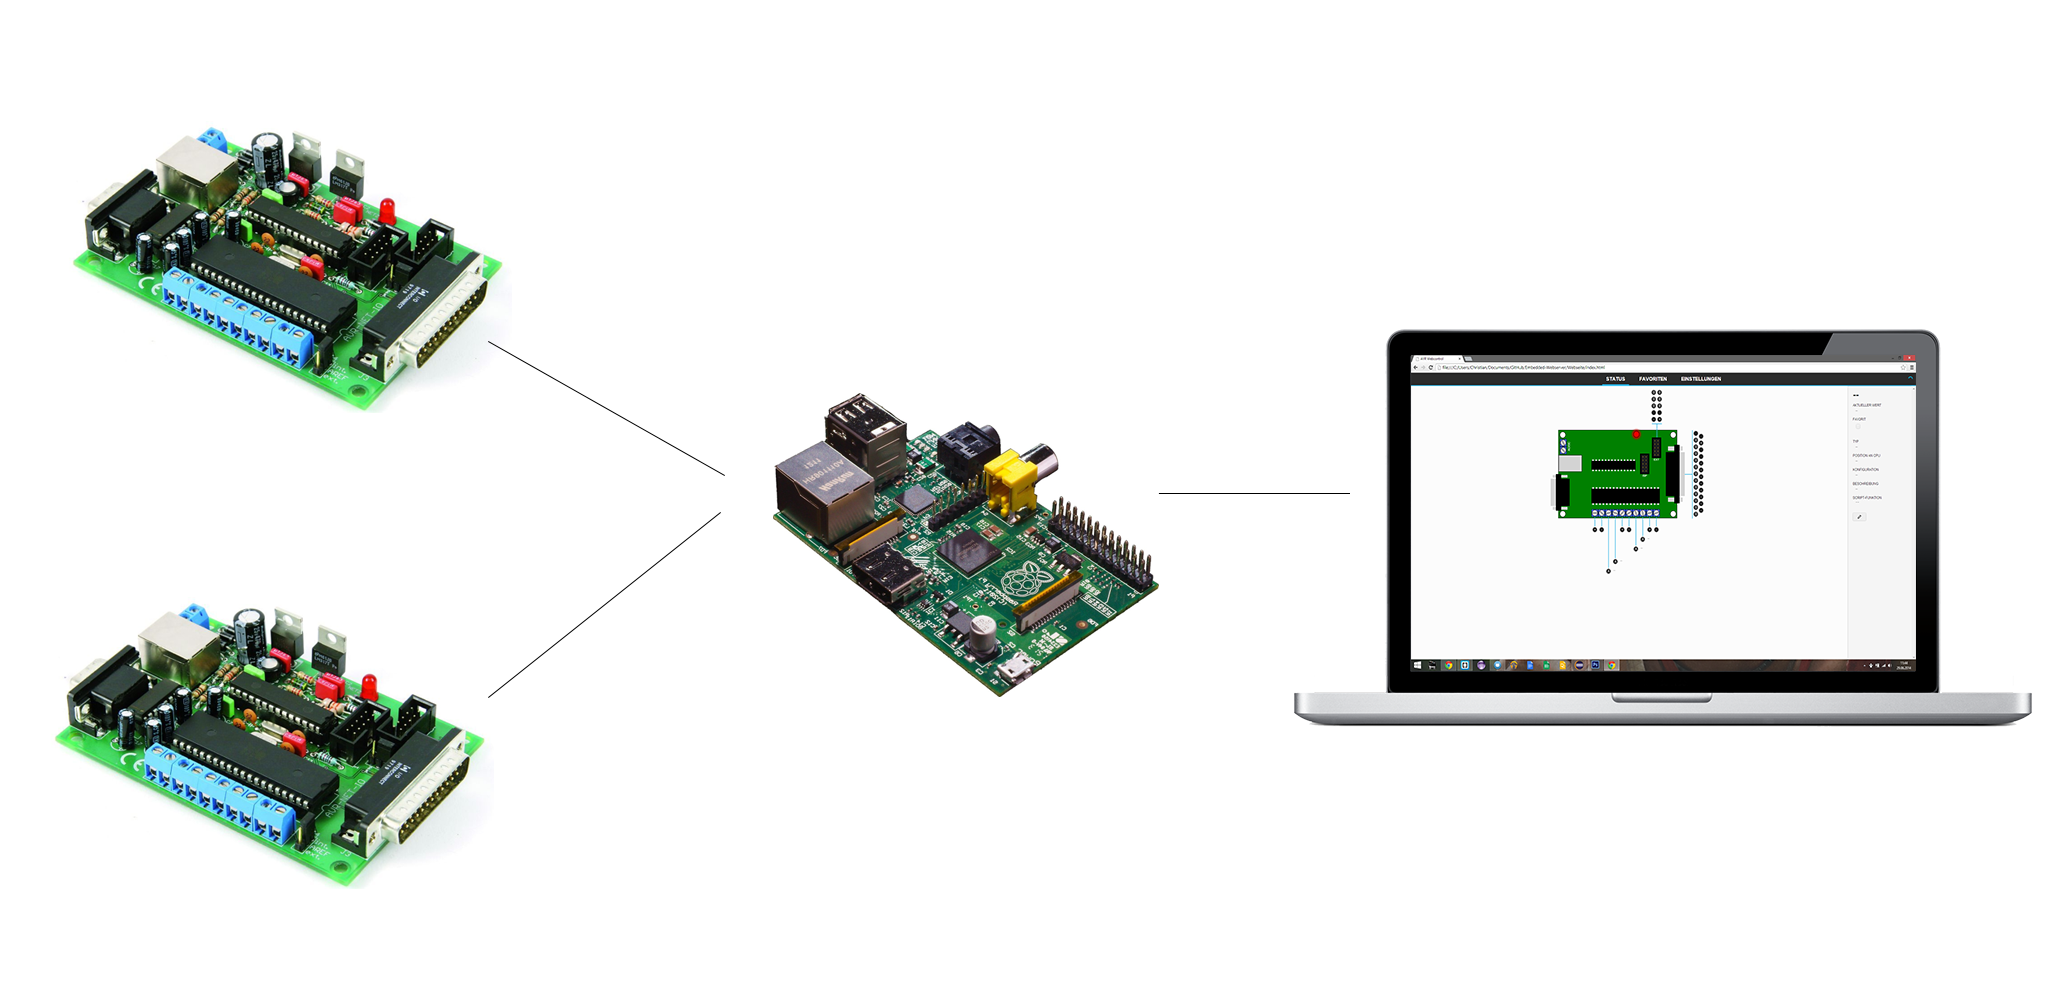
\includegraphics[width=13cm]{content/pictures/neues_system.png}
\caption[Schematischer Aufbau der Erweiterung]{Der grobe Aufbau des neues
Systems, links zwei Pollin Net-IO Boards, in der Mitte ein Rasberry Pi und links ein Client}
\label{struktur}
\end{figure}
Die Clients fragen alle Daten, welche in einer kleinen Datenbank
zwischengespeichert werden, von dem zentralen Rasberry Pi ab. So ergeben
sich zwei Teilsysteme: \\
\\
Das erste besteht aus dem Rasberry Pi und den Pollin Net-IO Boards,
welche über die von Pollin bereit gestellte Schnittstelle kommunizieren.
Die Verwendung der bereits vorhandenen Schnittstelle macht es unnötig am
Mikrocontroller irgendwelche Änderungen vorzunehmen oder eine neue Firmware
flashen zu müssen, was die Usability enorm steigert, da das System auch von
Laien betrieben werden kann. Sobald neue Werte vorliegen sollten die Pollin
Net-IO Boards die Änderungen zum Rasberry Pi pushen, welcher die Werte in einer
kleinen Datenbank zwischenspeichert.Zur Verwendung des bestehenden Protokolls 
muss dieses mit Wireshark analysiert und reverse engineered werden. Hierfür 
kann die Netzwerkkommunikation des Pollin Net-IO Boards mit der mitgeliferten 
PC-Software beobachtet werden.\\
\\
Das zweite System besteht aus dem Rasberry Pi und den Clients. Die Clients
fragen über HTTP beim Server die Webseiten-Dateien und Messwerte ab. Die
Messwerte sollten nicht wie bei der aktuellen Lösung gepollt sondern nur bei
Bedarf mit Hilfe der im Kapitel "`Technischer Hintergrund"' erläuterten HTML5
Server-Sent Events Technik zum Client gepusht werden. Dies reduziert den
unnötigen Netzwerkverkehr. Ein Client kann immer nur ein Pollin Net-IO Board
darstellen, deshalb muss dem Nutzer auf der Webseite die Möglichkeit gegeben
werden, das darzustellende Board auszuwählen. Außerdem muss auf der Webseite die
zu verwendenden Boards (also welche der Rasberry Pi anspricht und den Clients
anbietet) konfiguriert werden können. Ansonsten ist die Webseite ohne große
Änderungen übernehmbar.

%-----------------------------------------------------------------------------------------
\section{Änderungen an der Webseite/Server-Schnittstelle}
\label{aenderung_schnitstelle}
Die Kommunikation zwischen Server und Webseite muss für die neuen Anforderungen
entsprechend erweitert werden. \\
\\
In einem ersten Schritt sollten alle REST-URLs um einen Parameter erweitert
werden, der das Pollin Net-IO Board identifiziert, von dem die Informationen
angefordert werden. Dies ist nötig, da das System über mehrere Boards
verfügen könnte. Der Parameter kann als HTTP-GET Parameter übergeben werden. Als
ID eignet sich z.B. die IP-Adresse des betreffenden Boards oder eine künstliche 
ID in Form einer fortlaufend höheren Zahl. Die aufzurufende URL wäre folglich
z.B. \textrm{/rest/values?id=192.168.2.6}.\\
\\
Danach sollte das aktuell über die POST-Parameter stattfindende
Setzen von Pins ebenfalls über die REST-Schnittstelle gelöst werden. Hierfür
müssen zwei neue URLs eingeführt werden, eine zum Setzen der Pinwerte und eine
zum Setzen des DDRs. Natürlich müssen auch die neuen URLs über den
Parameter zum identifizieren des betroffnen Boards verfügen.\\
\\
Zum Schluss muss noch eine URL bereitgestellt werden um eine Liste aller
verfügbaren Boards abfragen zu können. Zusätzlich muss noch eine URL zum
Hinzufügen eines neuen Boards und eine zum Entfernen eines vorhandenen Boards
angelegt werden.\\
\\
Sobald an der Webseite die Schnitstelle manipuliert wird, ist die Kommunikation
mit dem von uns entwickelten Server nicht mehr möglich. Das System kann nicht
mit HTTP-GET Parametern umgehen. Aus diesem Grund sollte zu Beginn der
Entwicklung ein Testserver aufgesetzt werden. Dieser kann aus einem lokalen
XAMPP-Server bestehen, welcher statt dynamisch Dateien für die
REST-Schnittstelle zu erzeugen über statische Dateien verfügt, welche mit
Testwerten gefüllt sind. So würde z.B. unter \textrm{/rest/pininfo} eine reale
Datei liegen, in der anstatt der Platzhalter feste Werte eingetragen sind. Dies
ermöglicht die Entwicklung der Webseite bzw. dem Ansprechen des Servers ohne
einen funktionsfähigen Rasberry Pi.

%-----------------------------------------------------------------------------------------
\section{Änderungen an der Webseite}
\subsection{Einstellungen}
Die meisten Änderungen der Webseite finden in den JavaScript Dateien statt. Alle
Einstellungen werden mit Hilfe von \textrm{db.js} gespeichert. Aktuell werden
die Einstellungen lokal gespeichert. Dies kann entweder beibehalten werden oder
die Einstellungen können zentral auf dem Rasberry gespeichert werden, was es
ermöglichen würde Favoriten etc. zwischen mehreren Clients zu synchronisieren.
Hierfür müsste nur der Speicherort geändert werden, an dem \textrm{db.js} die
Daten ablegt. Anstatt diese lokal zu speichern müssten sie zum Server geschickt
werden, welcher sie wiederrum an alle anderen Clients weiterleitet.

\subsection{Implementierung der neuen Schnittstelle}
Die neue Schnittstelle zwischen Server und Webseite muss natürlich implementiert
werden. Alle hierfür nötigen Änderungen finden in der \textrm{rest.js} statt.
Neben der Implementierung der Server-Sent Events um neue Messwerte zu
empfangen müssen auch neue Getter und Setter angelegt werden, um z.B. alle
vorhandenen Boards abfragen zu können.\\
\\
Aktuell wird die Funktion \textrm{refreshValues()} dazu verwendet, die Daten
zyklisch nachzuladen. Gestartet wird dieser Vorgang von 
\textrm{startNewRefreshTask()}. Diese Funktionen können in Folge der Umstellung
auf Server-Sent Events komplett gelöscht werden. Wichtig ist hierbei, dass die
Fuktion \textrm{setOnValuesChanged()} und das Attribut
\textrm{onValuesChanged} beibehalten wird. Indem \textrm{onValuesChanged()}
aufgerufen wird, wird \textrm{ui.js} darüber informiert, dass sich die Messwerte
geändert haben, was zur Aktualisierung der Oberfläche führt.

\subsection{Scriptfunktionen}
Aktuell gibt es zwei verschiedene Typen von Skriptfunktionen. Für jeden Pin
lässt sich eine Skriptfunktion zum Erstellen des dargestellten Messwertes
hinterlegen. Diese Skriptfunktionen müssen nicht geändert werden.\\
\\
Zusätzlich gibt es eine Skrtipfunktion die in den Einstellungen festgelegt
werden kann. Sie muss für jedes Board separat verfügbar und anpassbar sein.
Aktuell wird sie auf dem Clientsystem als JavaScript ausgeführt, dass hat zu
Folge das die Skriptfunktion nur so lange funktioniert, wie das Clientsystem
aktiv ist, also die Webseite also angezeigt wird. Diese Skriptfunktion sollte auf dem
Rasberry Pi gespeichert und ausgeführt werden.

\subsection{Auswahl des darzustellenden Boards}
\label{auswahl_board}
Da die Webseite immer nur ein Pollin Net-IO Board darstellen kann, muss dem
Nutzer eine Möglichkeit gegeben werden, eines aus allen verfügbaren auszuwählen.
Hierfür bietet es sich an im \textrm{div} Element mit der ID \textrm{header}
ein \textrm{select} anzubieten (z.B. auf der linken Seite, siehe
Abbildung \ref{select_board}), mit dem das darzustellende Board ausgewählt
werden kann.
Für die Positionierung des Elementes kann das \textrm{div} Element mit der ID
\textrm{loading\_loop} als Vorlage genutzt werden.

\begin{figure}[H]
\centering
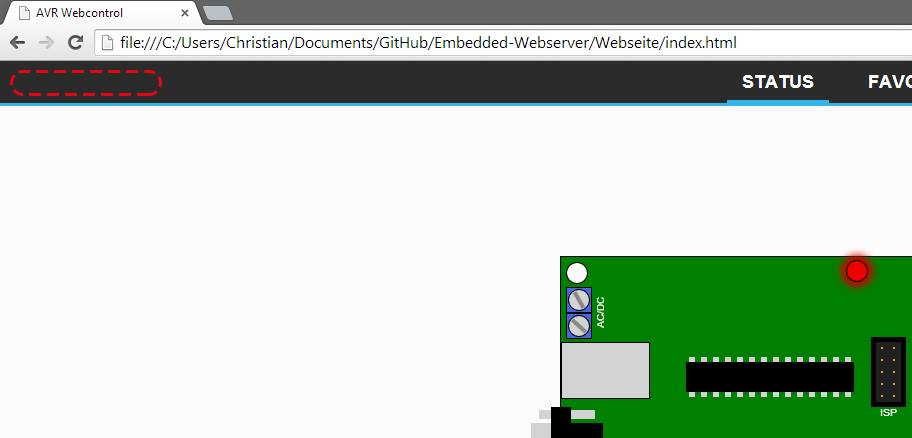
\includegraphics[width=13cm]{content/pictures/select_board.png}
\caption[Select Element]{Vorgeschalgene Position für ein select-Element um die
darzustellende Platine zu wählen}
\label{select_board}
\end{figure}

Beim Einfügen des \textrm{select} Elements in der Header ist zu beachten, dass die
Höhe des Headers nicht verändert werden sollte. Sollte dies dennoch nötig sein,
müssen die Kommentare im CSS-Code beachtet werden, um alle anderen nötigen
Änderungen durchzuführen.

\subsection{Verwaltung der Boards im System}
\label{verwaltung_system}
Im Einstellungs-Tab der Webseite muss eine Möglichkeit ergänzt werden, um die
neue Pollin Net-IO Boards zum System hinzuzufügen und vorhandene zu editieren
oder zu löschen. Für jedes Board sollte eine Sktipfunktion und ein Name
hinterlegbar sein. Der Name ermöglicht es dem Benutzer die Boards leichter
voneinander zu unterscheiden.

%-----------------------------------------------------------------------------------------
\section{Der neue Server}
Beim Server, welcher auf dem Rasberry Pi betrieben werden sollte, gibt es zwei
grundsätzliche Lösungsmöglichkeiten. Zum einen lässt sich der Server als
C/C++/Java-Programm realisieren, das einen Webserver zur Verfügung stellt oder
man realisiert den Server als PHP-Programm auf einem XAMPP-Server.\\
% Satz fängt mit "`zum einen"' an aber es kommt nie ein "`zum anderen"' ?? ..
\\
Bei beiden Alternativen muss der Server mit den einzelnen Pollin Net-IO Boards
kommunizieren, welche Daten über die REST-Schnittstelle bzw. die Server-Sent Events
bereitstellen sowie die Webseite hosten.

%-----------------------------------------------------------------------------------------
\section{Herangehensweise an das Projekt}
\subsection{Einpflegen des Rasberry Pi}
Im ersten Schritt sollte der Rasberry Pi in das bestehende System eingepflegt
werden. Hierfür sollte die Kommunikation zwischen Server und Webseite vorerst so
belassen werden wie sie aktuell ist, inklusive Polling. Der Server muss die
Daten von dem Pollin Net-IO Board empfangen (per Polling oder Pushing) und in
eine kleine Datenbank (oder ein Array etc.) hinterlegen. Bei jeder Abfrage der
Webseite werden die aktuellsten Daten weitergeleitet.\\
\\
Zu beachten ist, dass später die Skripte auf dem Server ausgeführt werden sollen.
Aus diesem Grund würde sich PHP als Programmiersprache anbieten, da PHP-Code,
der als Text vorliegt, direkt mit \textrm{eval()} ausgeführt werden kann.

\subsection{Betreiben mehrer Pollin Net-IO Boards}
Anschließend sollten mehrer Pollin Net-IO Boards betrieben werden können.
Hierfür muss die Server/Webseiten-Schnitstelle entsprechend dem Kapitel
\ref{aenderung_schnitstelle} überarbeitet werden. Die direkte Implementierung
der HTML5 Server-Sent Events ist empfehlenswert. Außerdem muss die Oberfläche
der Webseite um eine Auswahlmöglichkeit für das zu verwendende Board sowie eine
Konfigurationsmöglichkeit für die einzelnen Boards im System erweitert werden
(siehe Kapitel \ref{auswahl_board} und \ref{verwaltung_system}).

\subsection{Verlagern der Skriptfunktionen auf den Server}
Im letzten Schritt sollten die Skriptfunktionen, die nach jedem Neuladen der
Werte ausgeführt wird (aktuell im Settings-Tab einstellbar), auf dem Server
gespeichert und ausgeführt werden. Die Skriptfunktionen müssen natürlich von der
Webseite aus für jedes Board einzeln anpassbar sein. 
Wenn die Serverstruktur auf Basis des
XAMPP-Servers gewählt wurde, bietet sich PHP als Skriptsprache an, da der Code
nach dem Empfang neuer Werte direkt mit \textrm{eval()} ausgeführt werden kann.
Wichitg ist hierbei, dass über einfache Getter und Setter Funktionen der Zugriff
auf alle aktuellen Messwerte möglich ist und die Skriptfunktion auch Pins von
Boards sowie deren DDR manipulieren kann.
